\documentclass[a4paper]{article}
\addtolength{\hoffset}
{-2.25cm}
\addtolength{\textwidth}
{5cm}
\addtolength{\voffset}
{-3.25cm}
\addtolength{\textheight}
{5.5cm}
\setlength{\parskip}{0pt}
\setlength{\parindent}{0in}

\usepackage[utf8]{inputenc}
\usepackage{microtype}
\usepackage[english]{babel}
\usepackage{fancyhdr}
\usepackage{advdate}
\usepackage{enumitem}
\usepackage{amsmath, amssymb}
\usepackage{graphicx}
\usepackage{caption}
\usepackage{subcaption}
\usepackage{float}
\usepackage{titlesec}
\usepackage{wasysym}
\usepackage{url}
\usepackage{hyperref}
\usepackage{tikz, verbatimbox}
\usepackage{fixltx2e}
\usepackage{centernot}
\usepackage{algorithm}
\usepackage{algpseudocode}
\usepackage{listings}
\usetikzlibrary{shapes.geometric, arrows}
\usetikzlibrary{positioning}
\usepackage[table]{xcolor}

\graphicspath{{./static/}}
\tikzset{every picture/.style={line width=0.75pt}} %set default line width to 0.75pt

\newcommand{\LComment}[1]{\State \(\triangleright\) \text{#1}}
\MakeRobust{\Call}
\usepackage{pdfpages}

\newlength{\originalVOffset}
\newlength{\originalHOffset}
\setlength{\originalVOffset}{\voffset}   
\setlength{\originalHOffset}{\hoffset}

\begin{document}

\fancyhead[c]{}
\hrule \medskip
\begin{minipage}{0.195\textwidth}
\raggedright
Rishabh Indoria\\
21F3001823
\end{minipage}
\begin{minipage}{0.6\textwidth}
\centering
\LARGE
AI: Search Methods for Problem-Solving
\end{minipage}
\begin{minipage}{0.195\textwidth}
\raggedleft
\today \hfill \\
\end{minipage}
\medskip \hrule
\bigskip

\section{Introduction and History}

\subsection{Intelligent Agents}
\begin{itemize}
    \item \textbf{A First Course in Artificial Intelligence} by Deepak Khemani. First 7 chapters will be covered.
    \item \textbf{Intelligent Agents}: An entity that is persistent(it's there all the time), autonomous, proactive(decide what goals to achieve next) and goal directed(once it has goals, it will follow them). Human beings are also agents.
    \item An intelligent agent in a world carries a model of the world in its "head". the model may be an abstraction. A self-aware agent would model itself in the world model.
    \item Signal$\rightarrow$Symbol$\rightarrow$Signal
    \item Sense(Signal Processing) $\rightarrow$ Deliberate(Neuro fuzzy reasoning + Symbolic Reasoning) $\rightarrow$ Act(Output Signal)
    \begin{figure}[H]
        \centering
        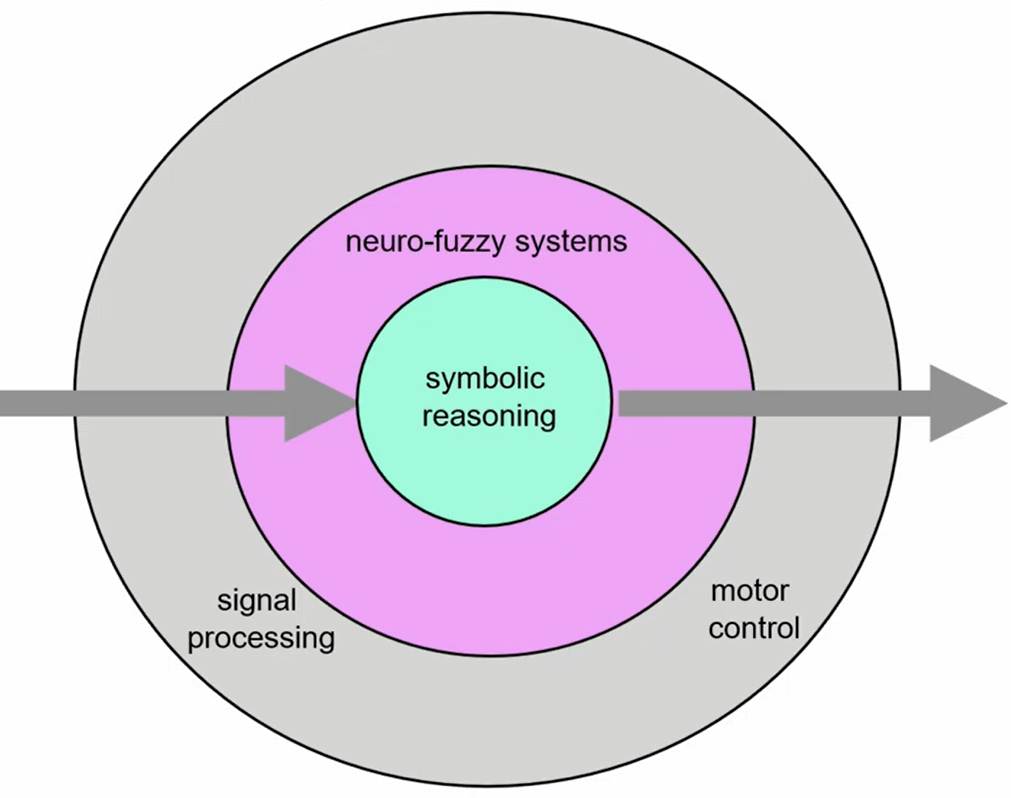
\includegraphics[width=0.5\linewidth]{Degree//static/AI_information_processing_view.png}
        \caption{Information Processing View of AI}
        \label{fig:AI-information-processing}
    \end{figure}
    \item \textbf{Intelligence}: \textbf{Remember the past and learn from it.} Memory and experience(case based reasoning), Learn a model(Machine learning), Recognize objects, faces, patterns(deep neural networks).\\
    \textbf{Understand the present. Be aware of the world around you.} Create a model of the world(knowledge representation), Make inferences from what you know(logic and reasoning).\\
    \textbf{Imagine the future. Work towards your goals.} Trial and error(heuristic search), Goals, plans, and actions(automated planning).
\end{itemize}

\subsection{Human Cognitive Architecture}
\begin{itemize}
    \item \textbf{Knowledge and Reasoning}: What does the agent know and what else does the agent know as a consequence of what it knows.
    \item \textbf{Semiotics}: A symbol is something that stands for something else. All languages, both spoken and written, are semiotic systems.
    \item \textbf{Biosemiotics}: How complex behaviour emerges when simple systems interact with each other through signs.
    \item \textbf{Reasoning}: The manipulation of symbols in a meaningful manner.
\end{itemize}

\subsection{Problem-Solving}
\begin{itemize}
    \item An autonomous agent in some world has a goal to achieve and a set of actions to choose from to strive for the goal.
    \item We deal with simple problems first, i.e., the world is static, the world is completely known, only one agent changes the world, action never fail, representation of the world is taken care of.
\end{itemize}

\section{Search Methods}

\subsection{State Space Search}
\begin{itemize}
    \item We start with the map coloring problem, where we want to color each region in the map with an allowed color such that no two adjacent regions have the same color.
    \begin{figure}[H]
        \centering
        \begin{subfigure}[b]{0.45\textwidth}
            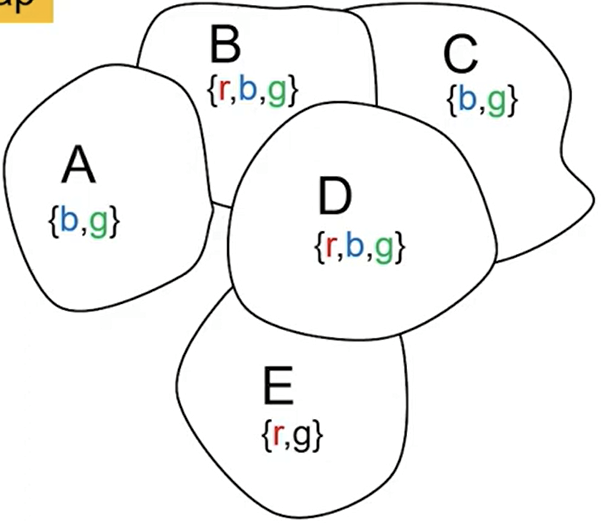
\includegraphics[width=1\textwidth]{Degree/static/AI_map_colors.png}
            \caption{Map with Constraints}
            \label{fig:AI-map-constraint}
        \end{subfigure}
        \hfill
        \begin{subfigure}[b]{0.45\textwidth}
            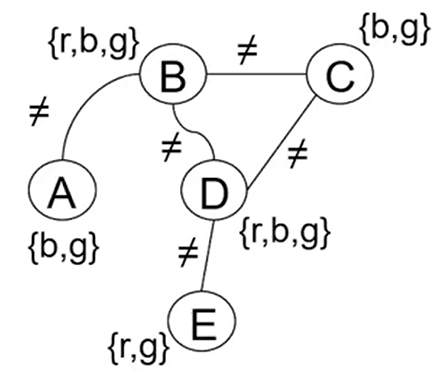
\includegraphics[width=1\textwidth]{Degree/static/AI_constraint_graph.png}
            \caption{Constraint Graph}
            \label{fig:AI-constraint-graph}
        \end{subfigure}
        \caption{Map Coloring Problem}
        \label{fig:AI-map-coloring-problem}
    \end{figure}
    \textbf{Brute Force}: Try all combinations of color for all regions.\\
    \textbf{Informed Search}: Choose a color that does not conflict with neighbors.\\
    \textbf{General Search}: Pose the problem to serve as an input to a general search algorithm.\\
    Map coloring can be posed as a constraint satisfaction problem or as a state space search, where the move is to assign a color to a region in a given partially colored state.
    \item \textbf{General Purpose methods}: Instead of writing a custom program for every problem to be solved, these aim to write search algorithms into which individual methods can be plugged in. One of them is State Space Search.
    \item \textbf{State or Solution Space Search}: Describe the given state, devise an operator to choose an action in each state, and then navigate the state space in search of the desired or goal state. Also known as Graph Search.\\
    A \textbf{state} is a representation of a situation.\\
    A \textit{MoveGen} function captures the moves that can be made in a given state.\\
    It returns a set of states - \textit{neighbors} - resulting from the moves.\\
    The state space is an implicit graph defined by the \textit{MoveGen} function.\\
    A \textit{GoalTest} function checks if the given state is a \textit{goal} state.\\
    A \textit{search algorithm} navigates the state space using these two functions.
    \item \textbf{The Water Jug Problem}: You have three jugs with capacity 8, 5 and 3 liters. Any state can be written as $[a,b,c]$, where $a,b,c$ are the amount of water present in each jug\\
    Start state: The 8-liter jug is filled with water, and the other two are empty, $[8,0,0]$. It can be seen that at any state the total amount of water remains the same.\\
    Goal: You are required to measure 4 liters of water. So, our goal state is $[4,x,y]$ or $[x,4,y]$ or $[x,y,4]$. A \textit{GoalTest} function can be written as
    \begin{algorithm}[H]
    \caption{GoalTest for the Water Jug Problem}\label{alg:AI-goal-test-water-jug}
        \begin{algorithmic}[1]
            \Require $[a,b,c]$, the state which needs to be checked
            \If{$a=4$ or $b=4$ or $c=4$}
                \State \Return True
            \EndIf
            \State \Return False
        \end{algorithmic}
    \end{algorithm}
    \item A few other examples are \textbf{The Eight Puzzle}, \textbf{The Man, Goat, Lion, Cabbage} and \textbf{The N-Queens Problem}.
\end{itemize}

\subsection{General Search Algorithms}
\begin{itemize}
    \item Searching is like treasure hunting. Our approach would be to generate and test where we traverse the space by generating new nodes and test each node whether it is the goal or not.
    \item \textbf{Simple Search 1}: Simply pick a node N from OPEN and check if it is the goal.
    \begin{algorithm}[H]
        \caption{Simple Search 1}\label{alg:AI-simple-search-1}
        \begin{algorithmic}[1]
            \LComment{S is the initial state}
            \State OPEN $\gets \{S\}$
            \While{\textit{OPEN} is not empty}
                \State pick some node N from OPEN
                \State OPEN $\gets$ OPEN - $\{n\}$
                \If{\Call{GoalTest}{N} = True}
                    \State \Return N
                \Else
                    \State OPEN $\gets$ OPEN $\cup$ \Call{MoveGen}{N}
                \EndIf
            \EndWhile
            \State \Return FAILURE
        \end{algorithmic}
    \end{algorithm}
    This algorithm may run into an infinite loop, to address it we have \textbf{Simple Search 2}.
    \begin{algorithm}[H]
        \caption{Simple Search 2}\label{alg:AI-simple-search-2}
        \begin{algorithmic}[1]
            \LComment{S is the initial state}
            \State OPEN $\gets \{S\}$
            \State CLOSED $\gets \{\}$ 
            \While{\textit{OPEN} is not empty}
                \State pick some node N from OPEN
                \State OPEN $\gets$ OPEN - $\{n\}$
                \State CLOSED $\gets$ CLOSED $\cup$ $\{N\}$
                \If{\Call{GoalTest}{N} = True}
                    \State \Return N
                \Else
                    \State OPEN $\gets$ OPEN $\cup$ $\{$\Call{MoveGen}{N} - CLOSED$\}$
                \EndIf
            \EndWhile
            \State \Return FAILURE
        \end{algorithmic}
    \end{algorithm}
    We can modify this a bit further by doing, OPEN $\gets$ OPEN $\cup$ $\{$\textit{MoveGen(N)} - CLOSED - OPEN$\}$, this lowers the state space even more.
\end{itemize}

\subsection{Planning and Configuration Problems}
\begin{itemize}
    \item \textbf{Planning Problems}: Goal is known or describe, path is sought. Examples include River crossing problems, route finding etc.
    \item \textbf{Configuration Problems}: A state satisfying a description is sought. Examples include N-queens, crossword puzzle, Sudoku, etc.
    \item The simple search algorithms will work for configuration problems, but they won't return any path.
    \item \textbf{NodePairs}: Keep track of parent nodes. Each node is a pair $(currentNode,\text{ }parentNode)$.
    \item \textbf{Depth First Search}: OPEN is a stack data structure
    \begin{algorithm}[H]
        \caption{Depth First Search}\label{alg:AI-DFS}
        \begin{algorithmic}[1]
            \State OPEN $\gets$ (S, null) : [ ]
            \State CLOSED $\gets$ [ ]
            \While{OPEN is not empty}
                \State nodePair $\gets$ head OPEN
                \State (N, $\_$) $\gets$ nodePair
                \If{\Call{GoalTest}{N} = True}
                    \State \Return \Call{ReconstructPath}{nodePair, CLOSED}
                \EndIf
                \State CLOSED $\gets$ nodePair : CLOSED
                \State children $\gets$ \Call{MoveGen}{N}
                \State newNodes $\gets$ \Call{RemoveSeen}{children, OPEN, CLOSED}
                \State newPairs $\gets$ \Call{MakePairs}{newNodes, N}
                \State OPEN $\gets$ newPairs ++ tail OPEN
            \EndWhile
            \State \Return [ ]
            \Statex
            \Function{RemoveSeen}{nodeList, OPEN, CLOSED}
                \If{nodeList = [ ]}
                    \State \Return [ ]
                \EndIf
                \State node $\gets$ head nodeList
                \If{\Call{OccursIn}{node, OPEN} or \Call{OccursIn}{node, CLOSED}}
                    \State \Return \Call{RemoveSeen}{tail nodeList, OPEN, CLOSED}
                \EndIf
                \State \Return node : \Call{RemoveSeen}{tail nodeList, OPEN, CLOSED}
            \EndFunction
            \Statex
            \Function{OccursIn}{node, nodePairs}
                \If{nodePairs = [ ]}
                    \State \Return FALSE
                \ElsIf{node = first head nodePairs}
                    \State \Return TRUE
                \EndIf
                \State \Return \Call{OccursIn}{node, tail nodePairs}
            \EndFunction
            \Statex
            \Function{MakePairs}{nodeList, parent}
                \If{nodeList = [ ]}
                    \State \Return [ ]
                \EndIf
                \State \Return (head nodeList, parent) : \Call{MakePairs}{tail nodeList, parent}
            \EndFunction
            \Statex
            \Function{ReconstructPath}{nodePair, CLOSED}
                \State (node, parent) $\gets$ nodePair
                \State path $\gets$ node : [ ]
                \While{parent is not null}
                    \State path $\gets$ parent : path
                    \State CLOSED $\gets$ \Call{SkipTo}{parent, CLOSED}
                    \State($\_$, parent) $\gets$ head CLOSED
                \EndWhile
                \State \Return path
            \EndFunction
            \algstore{bkbreak}
        \end{algorithmic}
    \end{algorithm}
    \begin{algorithm}[H]
        \caption{Depth First Search continued}
        \begin{algorithmic}
            \algrestore{bkbreak}
            \Statex
            \Function{SkipTo}{parent, nodePairs}
                \If{parent = first head nodePairs}
                    \State \Return nodePairs
                \EndIf
                \State \Return \Call{SkipTo}{parent, tail nodePairs}
            \EndFunction
        \end{algorithmic}
    \end{algorithm}
    \item \textbf{Breadth First Search}: We use a queue for the OPEN set.
    \begin{algorithm}
        \caption{Breadth First Search}\label{alg:AI-BFS}
        \begin{algorithmic}
            \State OPEN $\gets$ (S, null) : [ ]
            \State CLOSED $\gets$ [ ]
            \While{OPEN is not empty}
                \State nodePair $\gets$ head OPEN
                \State (N, $\_$) $\gets$ nodePair
                \If{\Call{GoalTest}{N} = True}
                    \State \Return \Call{ReconstructPath}{nodePair, CLOSED}
                \EndIf
                \State CLOSED $\gets$ nodePair : CLOSED
                \State children $\gets$ \Call{MoveGen}{N}
                \State newNodes $\gets$ \Call{RemoveSeen}{children, OPEN, CLOSED}
                \State newPairs $\gets$ \Call{MakePairs}{newNodes, N}
                \LComment{This is the only line that is different, we now add newPairs at the end of the list}
                \State OPEN $\gets$ tail OPEN ++ newPairs 
            \EndWhile
            \State \Return [ ]
        \end{algorithmic}
    \end{algorithm}
    \item BFS always generates the shortest path, whereas DFS may not generate the shortest path.
    \item \textbf{Time Complexity}: Assume constant branching factor $b$ and assume the goal occurs somewhere at depth $d$. In the best case the goal would be the first node scanned at depth $d$ and in the worst case the goal would b3 the last node scanned.\\
    Best Case: $N_{DFS}=d+1$ and $N_{BFS}=\frac{b^{d}-1}{b-1}+1$\\
    Worst Case: $N_{DFS}=N_{BFS}=\frac{b^{d+1}-1}{b-1}$\\
    Average: $N_{DFS}\approx \frac{b^d}{2}$ and $N_{BFS}\approx \frac{b^d(b+1)}{2(b-1)}$, $N_{BFS}\approx N_{DFS}(\frac{b+1}{b-1})$
    \begin{table}[H]
        \centering
        \begin{tabular}{|c|c|c|}
            \hline
             & Depth First Search & Breadth First Search \\
             \hline
            Time & Exponential & Exponential\\
            \hline
            Space & Linear & Exponential\\
            \hline
            Quality of Solution & No guarantees & Shortest path\\
            \hline
            Completeness & Not for infinite search space & Guaranteed to terminate if solution path exists\\
            \hline
        \end{tabular}
        \caption{DFS vs BFS}
        \label{tab:AI-DFS-vs-BFS}
    \end{table}
    \item \textbf{Depth Bounded DFS}: Do DFS with a depth bound $d$. It is not complete and does not guarantee the shortest path. Given below is a modified version that returns the count of nodes visited, to get the original version just remove count.
    \begin{algorithm}[H]
        \caption{Depth Bounded DFS}\label{alg:AI-depth-DFS}
        \begin{algorithmic}[1]
            \State count $\gets$ 0
            \State OPEN $\gets$ (S, null, 0) : [ ]
            \State CLOSED $\gets$ [ ]
            \While{OPEN is not empty}
                \State nodePair $\gets$ head OPEN
                \State (N, $\_$, depth) $\gets$ nodePair
                \If{\Call{GoalTest}{N} = True}
                    \State \Return count, \Call{ReconstructPath}{nodePair, CLOSED}
                \EndIf
                \State CLOSED $\gets$ nodePair : CLOSED
                \If{depth $<$ depthBound}
                    \State children $\gets$ \Call{MoveGen}{N}
                    \State newNodes $\gets$ \Call{RemoveSeen}{children, OPEN, CLOSED}
                    \State newPairs $\gets$ \Call{MakePairs}{newNodes, N, depth + 1}
                    \State OPEN $\gets$ newPairs ++ tail OPEN
                    \State count $\gets$ count + length newPairs
                \Else
                    \State OPEN $\gets$ tail OPEN
                \EndIf
            \EndWhile
            \State \Return count, [ ]
        \end{algorithmic}
    \end{algorithm}
    \item \textbf{Depth First Iterative Deepening}: Iteratively increase depth bound. Combines best of BFS and DFS. This will give the shortest path, but we have to be careful that we take correct nodes from CLOSED. $N_{DFID}\approx N_{BFD}\frac{b}{b-1}$ for large $b$.
    \begin{algorithm}[H]
        \caption{Depth First Iterative Deepening}\label{alg:AI-depth-first-iterative}
        \begin{algorithmic}[1]
            \State count $\gets$ $-1$
            \State path $\gets$ [ ]
            \State depthBound $\gets$ $0$
            \Repeat
                \State previousCount $\gets$ count
                \State (count, path) $\gets$ \Call{DB-DFS}{$S,depthBound$}
                \State depthBound $\gets$ depthBound $+1$
            \Until{(path is not empty) or (previousCount $==$ count)}
            \State \Return path
        \end{algorithmic}
    \end{algorithm}
    \item The monster that AI fights is Combinatorial Explosion.
    \item All these algorithms we studied are blind algorithms or uniformed search, they don't know where the goal is.
\end{itemize}

\subsection{Heuristic Search}
\begin{itemize}
    \item Testing the neighborhood and following the steepest gradient identifies which neighbors are the lowest or closest to the bottom.
    \item The heuristic function $h(N)$ is typically a user defined function, $h(Goal)=0$.
    \item \textbf{Best First Search}: Instead of having a simple stack or queue we use a priority queue sorted based on heuristic function. Search frontier depends upon the heuristic function. If graph is finite then this is complete and quality of solution will head towards the goal but may not give the shortest path.
    \begin{algorithm}[H]
        \caption{Best First Search}\label{alg:AI-BestFS}
        \begin{algorithmic}[1]
            \State OPEN $\gets$ (S, null, h(S)) : [ ]
            \State CLOSED $\gets$ [ ]
            \While{OPEN is not empty}
                \State nodePair $\gets$ head OPEN
                \State (N, $\_$, $\_$) $\gets$ nodePair
                \If{\Call{GoalTest}{N} = True}
                    \State \Return \Call{ReconstructPath}{nodePair, CLOSED}
                \EndIf
                \State CLOSED $\gets$ nodePair : CLOSED
                \State children $\gets$ \Call{MoveGen}{N}
                \State newNodes $\gets$ \Call{RemoveSeen}{children, OPEN, CLOSED}
                \State newPairs $\gets$ \Call{MakePairs}{newNodes, N}
                \State OPEN $\gets$ sort$_h$(newPairs ++ tail OPEN)
            \EndWhile
            \State \Return [ ]
        \end{algorithmic}
    \end{algorithm}
    \item For The eight puzzle we can define a few heuristic functions as follows:\\
    $h_1(n)=$ number of tiles out of place, Hamming distance.\\
    $h_2(n)=$ $\sum_{\text{for each tile}}$ Manhattan distance to its destination.
    \item \textbf{Hill Climbing}: A local search algorithm, i.e., move to the best neighbor if it is better, else terminate. In practice sorting is not needed, only the best node. This has burnt its bridges by not storing OPEN. We are interested in this because it is a constant space algorithm, which is a vast improvement on the exponential space for BFS and DFS. It's time complexity is linear. It treats the problem as an optimization problem.
    \begin{algorithm}[H]
        \caption{Hill Climbing}\label{alg:AI-hill-climbing}
        \begin{algorithmic}[1]
            \State node $\gets$ Start
            \State newNode $\gets$ head(sort$_h$(moveGen(node)))
            \While{ $h(newNode)<$ $h(node)$}
                \State node $\gets$ newNode
                \State newNode $\gets$ head(sort$_h$(moveGen(node)))
            \EndWhile
            \State \Return node
        \end{algorithmic}
    \end{algorithm}
\end{itemize}

\subsection{Escaping Local Optima}
\begin{itemize}
    \item \textbf{Solution Space Search}: Formulation of the search problem such that when we find the goal node we have the solution, and we are done.
    \item \textbf{Synthesis Methods}: Constructive methods. Starting with the initial state and build the solution state piece by piece.
    \item \textbf{Perturbation Methods}: Permutation of all possible candidate solutions.
    \item \textbf{SAT problem}: Given a boolean formula made up of a set of propositional variables $V=\{a,b,c,d,e,...\}$ each of which can be $true$ or $false$, or $1$ or $0$, to find an assignment of variables such that the given formula evaluates to $true$ or $1$.\\
    A SAT problem with $N$ variables has $2^N$ candidates.
    \item \textbf{Travelling Salesman Problem}: Given a set of cities and given a distance measure between every pair of cities, the task is to find a Hamiltonian cycle, visiting each city exactly once, having the least cost.
    \begin{enumerate}
        \item \textbf{Nearest Neighbor Heuristic}: Start at some city, move to nearest neighbor as long as it does not close the loop prematurely.
        \item \textbf{Greedy Heuristic}: Sort the edges, then add the shortest available edge to the tour as long as it does not close the loop prematurely.
        \item \textbf{Savings Heuristic}: Start with $n-1$ tours of length $2$ anchored on a base vertex and performs $n-2$ merge operations to construct the tour.
        \item \textbf{Perturbation operators}: Start with some tour, then choose two cities and interchange, this gives the solution space.
        \item \textbf{Edge Exchange}: Similar to above but now instead of choosing cities we are choosing edges. Can be $2$-edge exchange, $3$-edge, $4$-edge, etc. City exchange is a special case of $4$-edge exchange.
    \end{enumerate}
    \item Solution space of TSP grows in order factorial, much faster than SAT problem.
    \item A collection of problems with some solutions is available \href{http://comopt.ifi.uni-heidelberg.de/software/TSPLIB95/}{here}.
    \item To escape local minima we need something called \textbf{exploration}.
    \item \textbf{Beam Search}: Look at more than one option at each level. For a beam width $b$, look at best $b$ options. Heavily memory dependent.
    \item \textbf{Variable Neighborhood Descent}: Essentially we are doing hill climbing with different neighborhood functions. The idea is to use sparse functions before using denser functions, so the storage is not high. The algorithm assumes that there are $N$ $moveGen$ functions sorted according to the density of the neighborhoods produced.
    \begin{algorithm}[H]
        \caption{Variable Neighborhood Descent}\label{alg:Variable-Neighborhood-Descent}
        \begin{algorithmic}[1]
            \Statex \Call{VariableNeighbourhoodDescent}{ }
            \State $node\gets$ $start$
            \For{$i\gets$ $1$ to $n$}
                \State $moveGen\gets$ \Call{MoveGen}{$i$}
                \State $node\gets$ \Call{HillClimbing}{$node,moveGen$}
            \EndFor
            \State \Return $node$
        \end{algorithmic}
    \end{algorithm}
    \item \textbf{Best Neighbor}: Another variation of Hill Climbing, simply move to the best neighbor regardless of whether it is better than current node or not. This will require an external criterion to terminate. It will not escape local maxima, as once it escapes it will go right back to it in the next iteration.
    \begin{algorithm}[H]
        \caption{Best Neighbor}\label{alg:best-neighbor}
        \begin{algorithmic}[1]
            \Statex \Call{BestNeighbor}{ }
            \State $N\gets$ $start$
            \State $bestSeen\gets$ $N$
            \While{some termination criterion}
                \State $N\gets$ \Call{best}{$moveGen(N)$}
                \If{$N$ better than $bestSeen$}
                    \State $bestSeen\gets$ $N$
                \EndIf
            \EndWhile
            \State \Return $bestSeen$
        \end{algorithmic}
    \end{algorithm}
    \item \textbf{Tabu Search}: Similar to Best Neighbor but not allowed back immediately. An aspiration criterion can be added that says that if a tabu move result in a node that is better than bestSeen then it is allowed. To drive this search into newer areas, keep a frequency array and give preference to lower frequency bits or bits that have been changed less.
    \begin{algorithm}[H]
        \caption{Tabu Search}\label{alg:tabu-search}
        \begin{algorithmic}[1]
            \Statex \Call{TabuSearch}{ }
            \State $N\gets$ $start$
            \State $bestSeen\gets$ $N$
            \While{some termination criterion}
                \State $N\gets$ \Call{best}{\Call{allowed}{$moveGen(N)$}}
                \If{$N$ better than $bestSeen$}
                    \State $bestSeen\gets$ $N$
                \EndIf
            \EndWhile
            \State \Return $bestSeen$
        \end{algorithmic}
    \end{algorithm}
\end{itemize}

\end{document}